\chapter{Results and Discussion}

\section{Introduction}
This chapter presents the empirical findings, econometric evaluations, and theoretical interpretations resulting from the investigation into the value relevance of accounting information across the 2023 Nepalese commercial banking consolidation wave. The primary objective is to evaluate whether fundamental accounting numbers---specifically earnings per share (EPS) and book value per share (BVPS)---exhibit a statistically discernible association with secondary market equity prices observed immediately following statutory annual reporting deadlines ($\mathit{MPS}^{RD}$), and whether the valuation multiples attached to these accounting measures underwent a structural regime shift following the large-scale horizontal amalgamations executed in early 2023.

In accordance with the Faculty of Management, Tribhuvan University \textit{Master's Degree Dissertation Guidelines} (2019, pp.~14--15), the chapter is organized into two major substantive components: \textbf{Results} and \textbf{Discussion}.

The \textbf{Results} section (Section~4.2) details the empirical outcomes derived from the five sampled banking series over the six-year observation period (FY 2076/77 to FY 2081/82, corresponding to Gregorian years 2019/20 through 2024/25). The presentation proceeds through seven structured subsections:
\begin{enumerate}
    \item \textit{Descriptive Statistics} (Section~4.2.1), summarizing the distributional properties, central tendencies, and dispersions of the primary valuation variables across the full panel and comparative pre- and post-consolidation sub-periods;
    \item \textit{Correlation Analysis and Multicollinearity Assessment} (Section~4.2.2), examining bivariate linear associations, verifying collinearity boundaries between EPS and return on assets (ROA), and reviewing visual dispersion patterns;
    \item \textit{Baseline Value Relevance: Model 1 Estimation} (Section~4.2.3), reporting the estimation of Model~1 under two-way fixed effects with MacKinnon-White HC3 robust standard errors on Student's $t$ residual degrees of freedom;
    \item \textit{Impact of Consolidation on Value Relevance: Model 2 Estimation} (Section~4.2.4), detailing the estimation of Model~2, capturing pre-consolidation valuation slopes, regime interaction coefficients ($\delta_E, \delta_B$), implied post-consolidation net slopes, and the principal joint Wald test of parameter stability;
    \item \textit{Hypothesis Testing} (Section~4.2.5), evaluating the empirical findings against the four operational research hypotheses ($H_1, H_2, H_3, H_4$) formulated in Chapter~I;
    \item \textit{Robustness and Sensitivity Analyses (R1 through R8)} (Section~4.2.6), executing an eight-specification suite (R1--R2 baselines plus six robustness variants R3--R8) to probe the sensitivity of baseline estimates to profitability definitions, dividend exclusions, entity-timing mismatches, transition-year volatility, bonus share dilutive adjustments, and restated basic earnings; and
    \item \textit{Econometric Diagnostics and Specification Comparison} (Section~4.2.7), evaluating variance inflation factors (VIF), Breusch-Pagan heteroskedasticity tests, Cook's distance influence metrics, residual normality, and comparing pooled OLS, bank fixed effects, and two-way fixed effects specifications.
\end{enumerate}

For analytical transparency and audit traceability, the analytical figures embedded in this chapter correspond directly to verified analytical codebase outputs: Figure~\ref{fig:trends} maps to codebase asset F6, Figure~\ref{fig:scatter_matrix} to F1, Figure~\ref{fig:heatmap} to F2, Figure~\ref{fig:value_relevance} to F3, Figure~\ref{fig:coeff_forest} to F4, Figure~\ref{fig:robustness_forest} to A2, and Figure~\ref{fig:diagnostics} to F5.

The \textbf{Discussion} section (Section~4.3) evaluates, synthesizes, and critically interprets these empirical findings in the context of foundational valuation theory and contemporary empirical literature. It examines:
\begin{enumerate}
    \item The structural behavior of accounting valuation multiples in the pre-consolidation regime (Section~4.3.1);
    \item Economic and institutional interpretations of the downward shift in earnings multiples and the compression of book value multiples post-consolidation (Section~4.3.2);
    \item Theoretical reconciliation with the \citet{ohlson1995} residual income valuation framework, clean-surplus accounting, dividend signaling, and banking opacity theories (Section~4.3.3);
    \item Comparative alignment and divergence with prior Nepalese and emerging-market empirical literature (Section~4.3.4); and
    \item Methodological, institutional, and regulatory implications stemming from transition-year friction and statutory reporting deadlines under Section 59(2) of the Banks and Financial Institutions Act, 2017 (Section~4.3.5).
\end{enumerate}

\section{Results}

\subsection{Descriptive Statistics}
To establish the empirical baseline of the panel, Table~\ref{tab:t1_descriptives} reports the descriptive statistics---sample size ($n$), mean, standard deviation (SD), minimum, and maximum---for the dependent variable ($\mathit{MPS}^{RD}$) and explanatory accounting fundamentals (EPS, BVPS, DPS, and ROA) across the full analysis sample ($N = 28$) as well as the partitioned pre-consolidation ($n = 13$) and post-consolidation ($n = 15$) sub-periods.

The analysis sample consists of 28 realized bank-year observations from an intended balanced panel of 30 bank-years (5 commercial banks $\times$ 6 fiscal years). Two observations---Himalayan Bank Limited (HBL) for FY 2077/78 and Nepal Investment Mega Bank Limited (NIMB) for FY 2077/78---were dropped in strict adherence to the 5-day freshness rule defined in Chapter~III. Secondary market trading for both banking series was suspended during merger-related processes around the statutory reporting deadline (end of Chaitra 2078 BS / mid-April 2022), with trading resuming 54 days late (6 June 2022) for HBL and 47 days late (30 May 2022) for NIMB. In alignment with econometric protocol, these prices were recorded as missing rather than imputed, preserving data integrity.

\begin{table}[!htbp]
\centering
\small
\caption[Descriptive Statistics of Value-Relevance Variables]{Descriptive Statistics of Value-Relevance Variables, FY 2076/77--FY 2081/82}
\label{tab:t1_descriptives}
\begin{tabular}{llccccc}
\toprule
\textbf{Variable} & \textbf{Period} & \textbf{$n$} & \textbf{Mean} & \textbf{SD} & \textbf{Min} & \textbf{Max} \\
\midrule
$\mathit{MPS}^{RD}$ (NPR) & Full Sample & 28 & 254.34 & 98.82 & 136.90 & 520.00 \\
 & Pre-Consolidation & 13 & 310.59 & 119.46 & 176.00 & 520.00 \\
 & Post-Consolidation & 15 & 205.60 & 33.45 & 136.90 & 251.13 \\
\midrule
EPS (NPR) & Full Sample & 28 & 14.05 & 6.52 & 0.02 & 27.60 \\
 & Pre-Consolidation & 13 & 17.90 & 3.99 & 12.08 & 27.60 \\
 & Post-Consolidation & 15 & 10.72 & 6.53 & 0.02 & 22.06 \\
\midrule
BVPS (NPR) & Full Sample & 28 & 160.18 & 17.37 & 132.71 & 190.70 \\
 & Pre-Consolidation & 13 & 158.11 & 19.10 & 136.13 & 190.70 \\
 & Post-Consolidation & 15 & 161.97 & 16.18 & 132.71 & 190.40 \\
\midrule
DPS (NPR) & Full Sample & 28 & 3.56 & 3.98 & 0.00 & 12.50 \\
 & Pre-Consolidation & 13 & 6.06 & 3.56 & 2.00 & 12.50 \\
 & Post-Consolidation & 15 & 1.40 & 2.97 & 0.00 & 8.00 \\
\midrule
ROA (\%) & Full Sample & 28 & 0.99 & 0.47 & 0.00 & 1.79 \\
 & Pre-Consolidation & 13 & 1.31 & 0.22 & 0.90 & 1.79 \\
 & Post-Consolidation & 15 & 0.70 & 0.44 & 0.00 & 1.51 \\
\bottomrule
\end{tabular}

\vspace{4pt}
\begin{minipage}{\linewidth}
\footnotesize
\textit{Note.} Analysis sample: bank-years whose $\mathit{MPS}^{RD}$ falls within the 5-day trading window following the statutory annual reporting deadline, operationalized at the end of Chaitra (mid-April); the two window-excluded observations (HBL and NIMB FY 2077/78) are excluded and not imputed. Pre-consolidation = FY 2076/77--FY 2078/79 ($n = 13$); Post-consolidation = FY 2079/80--FY 2081/82 ($n = 15$). All monetary figures in Nepalese Rupees (NPR). Data recompiled from published annual reports and cross-checked aggregator market closing series.
\end{minipage}
\end{table}

The descriptive statistics in Table~\ref{tab:t1_descriptives} reveal substantial economic shifts across the pre- and post-consolidation periods:
\begin{enumerate}
    \item \textbf{Market Price ($\mathit{MPS}^{RD}$):} The full-sample mean closing share price at the reporting deadline was NPR 254.34, with a wide range spanning from NPR 136.90 to NPR 520.00. Across sub-periods, share prices experienced a substantial secular decline. In the pre-consolidation era (FY 2076/77--2078/79), the mean market price stood at NPR 310.59 (SD = 119.46), reaching a high of NPR 520.00 for HBL in FY 2076/77. Following the consolidation wave, the mean market price contracted to NPR 205.60 (SD = 33.45), representing an average price erosion of 33.80\% (NPR 104.99 per share). Concurrently, cross-sectional dispersion in share prices collapsed dramatically, with standard deviation falling by 72.00\% (from 119.46 to 33.45). This price compression is consistent with broader macroeconomic tightening in Nepal and a general market repricing of commercial bank equities toward a narrower valuation band.
    \item \textbf{Earnings per Share (EPS):} Across the full sample, EPS averaged NPR 14.05, ranging from a near-zero trough of NPR 0.02 (Kumari Bank in FY 2080/81) to an apex of NPR 27.60 (HBL in FY 2076/77). Between regimes, mean EPS declined from NPR 17.90 in the pre-consolidation period to NPR 10.72 post-consolidation---a contraction of 40.11\%. Unlike market prices, the dispersion of earnings expanded substantially post-consolidation: the standard deviation increased from 3.99 to 6.53 (+63.66\%). This divergence is consistent with post-merger integration dynamics---marked by non-performing loan (NPL) recognition, provisioning burdens, and harmonization adjustments---which coincided with substantial earnings volatility across surviving entities.
    \item \textbf{Book Value per Share (BVPS):} In marked contrast to market prices and earnings, book value per share exhibited remarkable stability across regimes. The full-sample mean BVPS was NPR 160.18 (SD = 17.37), bounded between NPR 132.71 and NPR 190.70. Across sub-periods, mean BVPS rose slightly from NPR 158.11 (SD = 19.10) pre-consolidation to NPR 161.97 (SD = 16.18) post-consolidation---a modest upward increment of 2.44\% (NPR 3.86). The relative stability of BVPS is compatible with the accumulation of statutory reserves and regulatory capital requirements mandated by NRB, even during periods of cash dividend suspensions.
    \item \textbf{Dividend per Share (DPS):} Cash dividend distributions experienced a sharp contraction. In the pre-consolidation period, all sampled banks distributed cash dividends, yielding a mean DPS of NPR 6.06 (SD = 3.56; ranging from NPR 2.00 to NPR 12.50). In the post-consolidation era, mean DPS plummeted to NPR 1.40 (SD = 2.97), representing a 76.90\% reduction. Across the 15 post-consolidation bank-years, 12 observations recorded exactly zero cash dividends, coinciding with heightened regulatory capital conservation, elevated credit-loss provisioning, and dividend withholding to preserve capital adequacy ratios.
    \item \textbf{Return on Assets (ROA):} Operating profitability halved across the structural divide. Full-sample mean ROA stood at 0.99\% (SD = 0.47\%). Pre-consolidation ROA averaged 1.31\% (SD = 0.22\%, range 0.90\% to 1.79\%), whereas post-consolidation ROA dropped to 0.70\% (SD = 0.44\%, range 0.00\% to 1.51\%)---a 46.56\% decline.
\end{enumerate}

To illustrate these longitudinal trajectories across each sampled institution, Figure~\ref{fig:trends} plots the time-series trends for all five variables by bank series across the six fiscal years.

\begin{figure}[!htbp]
\centering
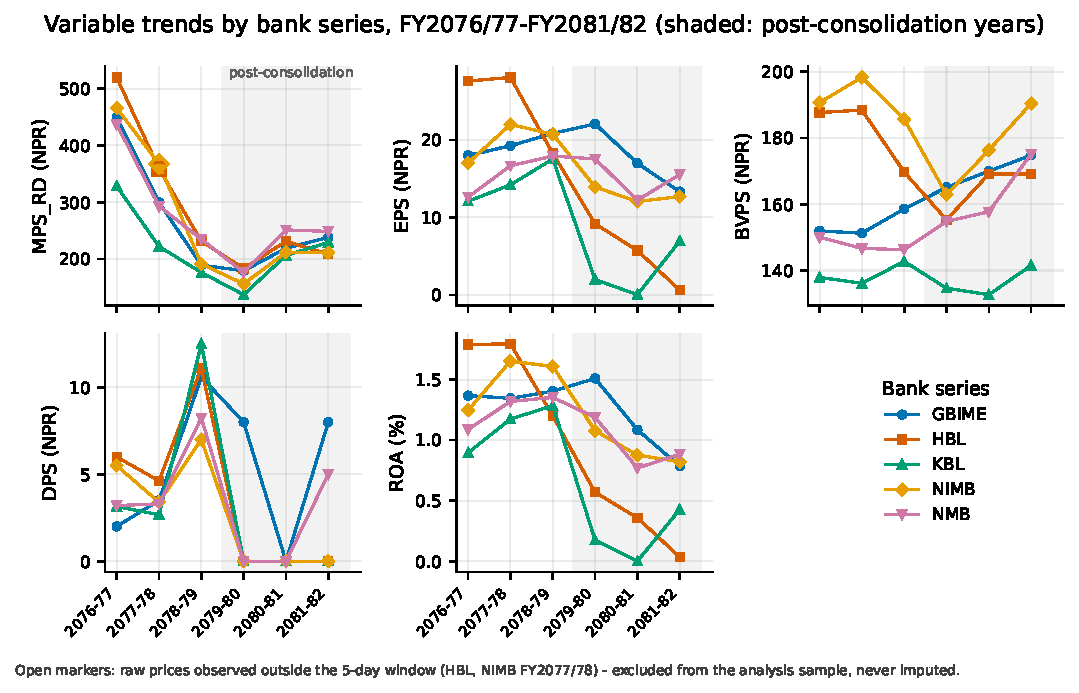
\includegraphics[width=0.92\textwidth]{figures/F6_trends.pdf}
\caption{Variable Trends by Bank Series across FY 2076/77--FY 2081/82}
\label{fig:trends}
\vspace{2pt}
\begin{minipage}{\linewidth}
\footnotesize
\textit{Note.} Variable trends across the six fiscal years (FY 2076/77 through FY 2081/82) for Global IME Bank Limited (GBIME), Himalayan Bank Limited (HBL), Kumari Bank Limited (KBL), Nepal Investment Mega Bank Limited (NIMB), and NMB Bank Limited (NMB). The shaded region delineates the post-consolidation regime (FY 2079/80--FY 2081/82). Window-excluded prices for HBL and NIMB in FY 2077/78 are represented as open markers. The connecting lines pass continuously through the excluded periods; the open markers designate observations excluded from regression estimation under the freshness rule (Codebase Asset F6).
\end{minipage}
\end{figure}

As visually depicted in Figure~\ref{fig:trends}, the post-consolidation shaded window coincides with a synchronized contraction in market share prices ($\mathit{MPS}^{RD}$), a steep downward break in earnings per share (EPS), and a virtual cessation of dividend payouts (DPS), whereas book value per share (BVPS) remained anchored across the structural divide.

\subsection{Correlation Analysis and Multicollinearity Assessment}
Table~\ref{tab:t2_correlations} reports the Pearson correlation coefficients among the dependent variable and explanatory financial indicators across the 28 realized observations.

\begin{table}[!htbp]
\centering
\small
\caption{Pearson Correlation Matrix of Value-Relevance Variables ($N = 28$)}
\label{tab:t2_correlations}
\begin{tabular}{lccccc}
\toprule
\textbf{Variable} & \textbf{$\mathit{MPS}^{RD}$} & \textbf{EPS} & \textbf{BVPS} & \textbf{DPS} & \textbf{ROA} \\
\midrule
$\mathit{MPS}^{RD}$ & 1.000 &  &  &  &  \\
EPS & 0.358 & 1.000 &  &  &  \\
BVPS & 0.217 & 0.372 & 1.000 &  &  \\
DPS & 0.082 & 0.612\textsuperscript{**} & 0.129 & 1.000 &  \\
ROA & 0.378\textsuperscript{*} & 0.975\textsuperscript{**} & 0.278 & 0.595\textsuperscript{**} & 1.000 \\
\bottomrule
\end{tabular}

\vspace{4pt}
\begin{minipage}{\linewidth}
\footnotesize
\textit{Note.} \textsuperscript{*} $p < 0.05$, \textsuperscript{**} $p < 0.01$ (two-tailed). Analysis sample of 28 realized bank-year observations. Price-to-Earnings (P/E) ratio is excluded by construction due to mechanical endogeneity with Market Price per Share at Reporting Deadline ($\mathit{MPS}^{RD}$).
\end{minipage}
\end{table}

The correlation matrix reveals several key empirical patterns:
\begin{enumerate}
    \item \textbf{Unconditional Price Associations:} In raw, unadjusted bivariate correlations, $\mathit{MPS}^{RD}$ exhibits a positive correlation with EPS ($r = 0.358, p = 0.061$) and BVPS ($r = 0.217, p = 0.268$). Although positive---consistent with general equity valuation logic---neither bivariate association achieves statistical significance at the 5\% level in the unadjusted bivariate sample. Operating profitability (ROA) displays a statistically significant positive bivariate correlation with market price ($r = 0.378, p = 0.047$), whereas cash dividend per share (DPS) exhibits an extraordinarily weak linear correlation ($r = 0.082, p = 0.678$).
    \item \textbf{Severe Collinearity between EPS and ROA:} Crucially, the Pearson correlation coefficient between EPS and ROA is $r = 0.975$ ($p < 0.001$). Entering both regressors simultaneously into a multivariate linear specification would generate severe variance inflation ($\text{VIF} \approx 1 / (1 - 0.975^2) \approx 20.2$), severely destabilizing standard errors, inducing sign reversals, and invalidating inference. Consequently, ROA is strictly excluded from concurrent inclusion with EPS in all econometric specifications; it is deployed exclusively as a substitute operating profitability regressor in robustness specification R3.
    \item \textbf{Core Regressor Independence:} In contrast, the bivariate correlation between the two core explanatory variables of the Ohlson framework---EPS and BVPS---is moderate ($r = 0.372, p = 0.051$). This demonstrates that earnings and book value capture distinct dimensions of financial performance and equity value, retaining sufficient independent variation for simultaneous estimation without multicollinearity distortion.
\end{enumerate}

Figure~\ref{fig:scatter_matrix} presents the bivariate scatter plot matrix among the primary value-relevance variables ($\mathit{MPS}^{RD}$, EPS, and BVPS), while Figure~\ref{fig:heatmap} illustrates the corresponding correlation heatmap.

\begin{figure}[!htbp]
\centering
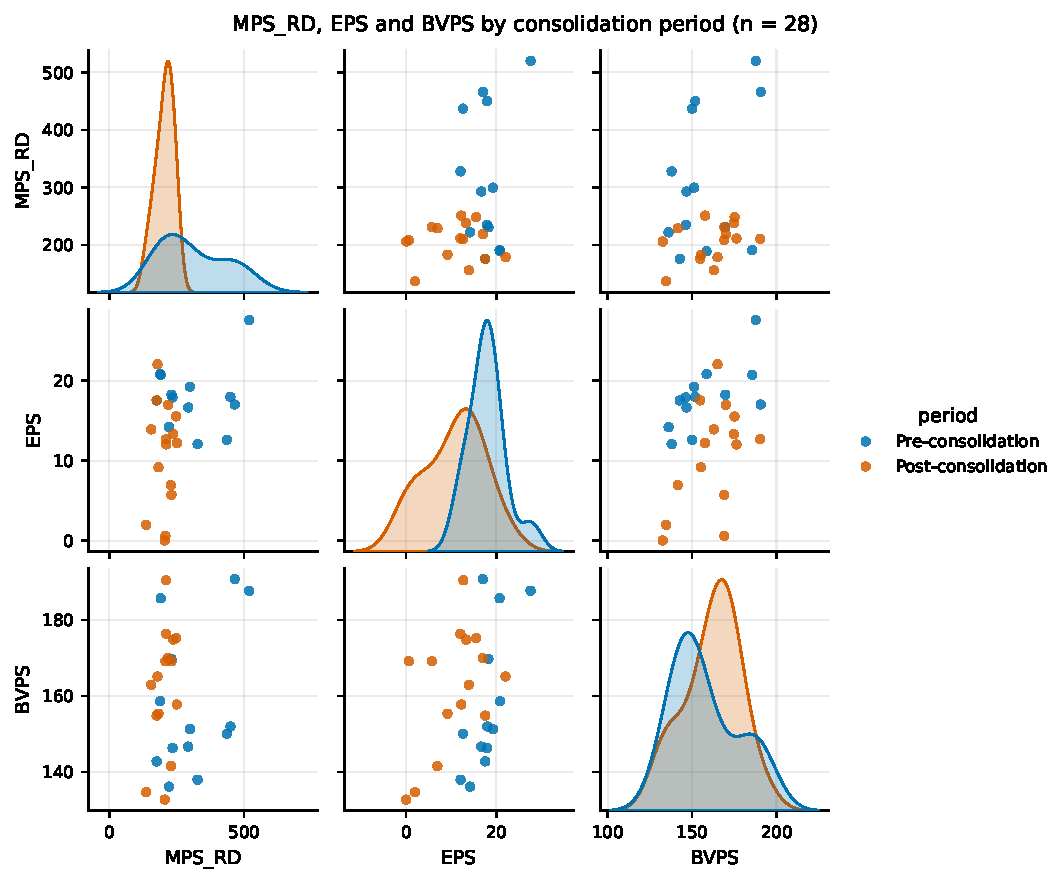
\includegraphics[width=0.88\textwidth]{figures/F1_scatter_matrix.pdf}
\caption{Bivariate Scatter Plot Matrix of Value-Relevance Variables}
\label{fig:scatter_matrix}
\vspace{2pt}
\begin{minipage}{\linewidth}
\footnotesize
\textit{Note.} Pairwise scatter plots and univariate kernel density distributions for $\mathit{MPS}^{RD}$, EPS, and BVPS across the realized panel ($N = 28$) (Codebase Asset F1).
\end{minipage}
\end{figure}

\begin{figure}[!htbp]
\centering
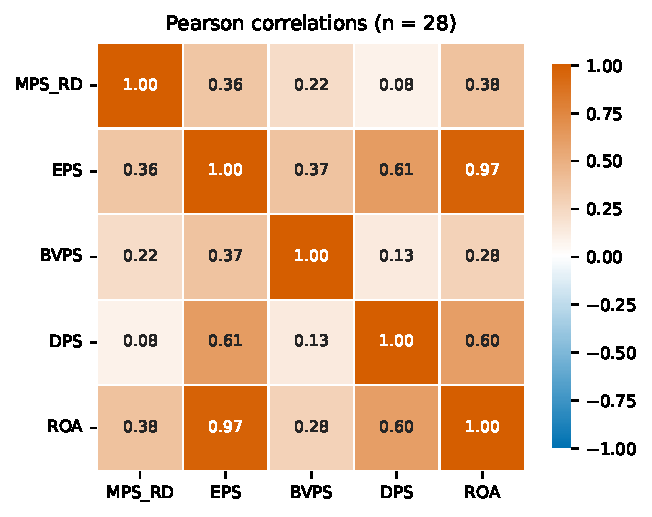
\includegraphics[width=0.72\textwidth]{figures/F2_correlation_heatmap.pdf}
\caption{Pearson Correlation Heatmap of Value-Relevance Variables}
\label{fig:heatmap}
\vspace{2pt}
\begin{minipage}{\linewidth}
\footnotesize
\textit{Note.} Correlation heatmap displaying pairwise Pearson correlation coefficients among value-relevance variables across the realized panel ($N = 28$) (Codebase Asset F2).
\end{minipage}
\end{figure}

\subsection{Baseline Value Relevance: Model 1 Estimation}
To address Research Question~1 and provide an empirical benchmark of accounting value relevance prior to evaluating regime shifts, Model~1 estimates the static Ohlson valuation equation across the entire six-year panel:
\begin{equation}
\mathit{MPS}^{RD}_{it} = \alpha + \mu_i + \lambda_t + \beta_E \mathit{EPS}_{it} + \beta_B \mathit{BVPS}_{it} + \varepsilon_{it}
\end{equation}
where $\alpha$ is the constant baseline intercept, $\mu_i$ represents unobserved time-invariant bank fixed effects (with GBIME serving as reference bank), and $\lambda_t$ represents common fiscal-year fixed effects (with FY 2076/77 serving as reference year). Standard errors, $t$-statistics, $p$-values, and confidence intervals are estimated using \citet{mackinnon1985} HC3 heteroskedasticity-consistent standard errors evaluated on Student's $t$ distribution with residual degrees of freedom ($\text{df} = 16$).

Table~\ref{tab:t3_model1} reports the parameter estimates for Model~1, with MacKinnon-White HC3 robust standard errors in parentheses beneath each estimate; $t$-statistics, $p$-values, and 95\% confidence intervals are reported in the text.

\begin{table}[!htbp]
\centering
\small
\caption{Model 1: Baseline Value Relevance of Accounting Fundamentals ($N = 28$)}
\label{tab:t3_model1}
\begin{tabular}{>{\raggedright\arraybackslash}p{0.38\textwidth}>{\raggedleft\arraybackslash}p{0.32\textwidth}}
\toprule
\textbf{Independent Variable} & \textbf{Dependent Variable: $\mathit{MPS}^{RD}$} \\
\midrule
Earnings per Share (EPS) & 2.095 \\
& (4.096) \\
Book Value per Share (BVPS) & 0.219 \\
& (1.858) \\
\addlinespace
\multicolumn{2}{l}{\textbf{Fixed Effects}} \\
\addlinespace
Bank Fixed Effects ($\mu_i$) & Yes \\
Fiscal-Year Fixed Effects ($\lambda_t$) & Yes \\
\addlinespace
\multicolumn{2}{l}{\textbf{Model Diagnostics}} \\
\addlinespace
Observations ($N$) & 28 \\
$R^2$ (LSDV) & 0.948 \\
Adjusted $R^2$ & 0.912 \\
Within-$R^2$ & 0.152 \\
Residual Degrees of Freedom & 16 \\
\bottomrule
\end{tabular}

\vspace{4pt}
\begin{minipage}{\linewidth}
\footnotesize
\textit{Note.} Dependent variable: Market Price per Share at Reporting Deadline ($\mathit{MPS}^{RD}$). OLS estimation with two-way fixed effects (bank dummies and fiscal-year dummies). MacKinnon-White HC3 robust standard errors in parentheses beneath parameter estimates. Bank fixed effects include 4 dummies (reference: GBIME); fiscal-year fixed effects include 5 dummies (reference: FY 2076/77). $R^2$ (LSDV) is the least-squares dummy-variable fit including fixed effects; Within-$R^2$ is the share of bank-and-year-adjusted variation explained by the slopes. Parameter count: 1 intercept + 4 bank dummies + 5 year dummies + 2 slopes = 12 parameters; residual degrees of freedom: $28 - 12 = 16$. Two-tailed tests at 5\% significance level; $t$-statistics, $p$-values, and 95\% confidence intervals are reported in the text.
\end{minipage}
\end{table}

The baseline results in Table~\ref{tab:t3_model1} provide important empirical insights:
\begin{enumerate}
    \item \textbf{Coefficient Magnitudes and Signs:} Both accounting fundamentals exhibit positive coefficients: $\beta_E = 2.095$ and $\beta_B = 0.219$. In economic terms, this suggests that across the full observation span, each additional NPR 1.00 of reported earnings per share is associated with an incremental NPR 2.10 in post-deadline market share price, while each additional NPR 1.00 of book equity per share is associated with an incremental NPR 0.22 in market price, holding unobserved bank characteristics and common macro-temporal shocks constant.
    \item \textbf{Statistical Significance under Robust Inference:} Neither slope coefficient achieves statistical significance at conventional levels. For EPS, the $t$-statistic is $0.51$ ($p = 0.616$ on $t(16)$), and the 95\% HC3 confidence interval spans widely from NPR $-6.587$ to NPR $10.777$. For BVPS, the $t$-statistic is $0.12$ ($p = 0.908$ on $t(16)$), with a 95\% confidence interval spanning from NPR $-3.720$ to NPR $4.158$.
    \item \textbf{Goodness of Fit and Degrees of Freedom:} The model exhibits a high coefficient of determination ($R^2 = 0.948$, Adjusted $R^2 = 0.912$). However, as demonstrated in the specification comparisons in Section~4.2.7, this high explanatory power is almost entirely driven by the two-way fixed effects structure---specifically the fiscal-year dummies ($\lambda_t$), which absorb the substantial macro-market repricing of NEPSE over this period. Accounting for 1 constant intercept, 4 bank dummy parameters, 5 fiscal-year dummy parameters, and 2 slope regressors consumes 12 degrees of freedom, leaving exactly $28 - 12 = 16$ residual degrees of freedom.
\end{enumerate}

\subsection{Impact of Consolidation on Value Relevance: Model 2 Estimation}
To evaluate Research Question~2 and directly test whether the 2023 consolidation wave altered the valuation relationship between accounting fundamentals and equity prices, Model~2 introduces consolidation interaction terms into the two-way fixed effects framework:
\begin{equation}
\begin{aligned}
\mathit{MPS}^{RD}_{it} ={}& \alpha + \mu_i + \lambda_t + \beta_E \mathit{EPS}_{it} + \beta_B \mathit{BVPS}_{it} \\
& + \delta_E (\mathit{EPS}_{it} \times \mathit{Post}_t) + \delta_B (\mathit{BVPS}_{it} \times \mathit{Post}_t) + \varepsilon_{it}
\end{aligned}
\end{equation}
where $\mathit{Post}_t = 1$ for the post-consolidation fiscal years (FY 2079/80, 2080/81, and 2081/82) and $\mathit{Post}_t = 0$ for the pre-consolidation fiscal years (FY 2076/77, 2077/78, and 2078/79). Reference categories remain identical (GBIME for $\mu_i$, FY 2076/77 for $\lambda_t$).

Because common fiscal-year fixed effects ($\lambda_t$) are fully specified, the stand-alone indicator $\mathit{Post}_t$ is an exact linear combination of the fiscal-year dummies ($\mathit{Post}_t = D_{2079/80} + D_{2080/81} + D_{2081/82}$); consequently, the main effect of $\mathit{Post}_t$ is perfectly absorbed by the year fixed effects and cannot be separately estimated. The pre-consolidation valuation slopes are captured by $\beta_E$ and $\beta_B$, the regime interaction coefficients are captured by $\delta_E$ and $\delta_B$, and the implied post-consolidation valuation slopes are given by the linear combinations $(\beta_E + \delta_E)$ and $(\beta_B + \delta_B)$.

Table~\ref{tab:t4_model2} reports the estimation results for Model~2, including pre-consolidation slopes, interaction shifts, implied post-consolidation slopes, and the principal joint Wald test of structural parameter change, with MacKinnon-White HC3 robust standard errors in parentheses beneath each estimate on Student's $t$ distribution ($\text{df} = 14$); $t$-statistics, $p$-values, and confidence intervals are reported in the text.

\begin{table}[!htbp]
\centering
\small
\caption{Model 2: Value Relevance Regime Shift Across Consolidation ($N = 28$)}
\label{tab:t4_model2}
\begin{tabular}{>{\raggedright\arraybackslash}p{0.38\textwidth}>{\raggedleft\arraybackslash}p{0.32\textwidth}}
\toprule
\textbf{Model Parameter / Term} & \textbf{Dependent Variable: $\mathit{MPS}^{RD}$} \\
\midrule
\multicolumn{2}{l}{\textbf{Pre-Consolidation Slopes}} \\
\addlinespace
Earnings per Share ($\beta_E$) & 5.577 \\
& (3.560) \\
Book Value per Share ($\beta_B$) & 0.100 \\
& (1.306) \\
\addlinespace
\multicolumn{2}{l}{\textbf{Consolidation Interaction Shifts}} \\
\addlinespace
EPS $\times$ Post ($\delta_E$) & $-3.124$ \\
& (4.003) \\
BVPS $\times$ Post ($\delta_B$) & $-1.758$ \\
& (1.231) \\
\addlinespace
\multicolumn{2}{l}{\textbf{Implied Post-Consolidation Slopes}} \\
\addlinespace
Implied EPS Slope ($\beta_E + \delta_E$) & 2.453 \\
& (2.269) \\
Implied BVPS Slope ($\beta_B + \delta_B$) & $-1.658$ \\
& (1.120) \\
\addlinespace
\multicolumn{2}{l}{\textbf{Diagnostics and Structural Change Tests}} \\
\addlinespace
Wald Test: $F(2, 14)$ \newline $[H_0: \delta_E = \delta_B = 0]$ & 2.954 ($p = 0.085$) \\
Bank Fixed Effects ($\mu_i$) & Yes \\
Fiscal-Year Fixed Effects ($\lambda_t$) & Yes \\
Observations ($N$) & 28 \\
$R^2$ (LSDV) & 0.978 \\
Within-$R^2$ & 0.642 \\
Residual Degrees of Freedom & 14 \\
\bottomrule
\end{tabular}

\vspace{4pt}
\begin{minipage}{\linewidth}
\footnotesize
\textit{Note.} Dependent variable: $\mathit{MPS}^{RD}$. OLS estimation with bank and fiscal-year fixed effects. Post indicator equals 1 for FY 2079/80--2081/82 and 0 for FY 2076/77--2078/79; stand-alone Post main effect is fully absorbed by the fiscal-year fixed effects. MacKinnon-White HC3 robust standard errors in parentheses beneath parameter estimates. Bank fixed effects include 4 dummies (reference: GBIME); fiscal-year fixed effects include 5 dummies (reference: FY 2076/77). $R^2$ (LSDV) is the least-squares dummy-variable fit including fixed effects; Within-$R^2$ is the share of bank-and-year-adjusted variation explained by the slopes and interactions. Implied post-consolidation slopes are linear combinations evaluated under the HC3 covariance. Residual degrees of freedom: $28 - 14 = 14$. Two-tailed $t$-tests for individual parameters; right-tail Wald $F$-test for joint hypothesis; the Wald test is marginally significant at the 10\% level. $t$-statistics, $p$-values, and confidence intervals are reported in the text.
\end{minipage}
\end{table}

The empirical estimates in Table~\ref{tab:t4_model2} provide substantive evidence regarding structural changes in valuation dynamics:
\begin{enumerate}
    \item \textbf{Pre-Consolidation Valuation Regime:}
    \begin{itemize}
        \item Prior to the 2023 consolidation wave, the estimated valuation slope for earnings per share was $\beta_E = 5.577$ (HC3 SE = 3.560, $t = 1.57, p = 0.140$). In economic magnitude, equity investors priced commercial bank shares at approximately 5.58 times reported earnings per share. While economically substantial, this estimate is not statistically significant at the 5\% level ($p = 0.140$ on $t(14)$), reflecting the wide confidence interval ([-2.059, 13.213]) resulting from small sample degrees of freedom and conservative HC3 standard errors.
        \item The pre-consolidation slope for book value per share was negligible: $\beta_B = 0.100$ (HC3 SE = 1.306, $t = 0.08, p = 0.940$). In the pre-consolidation environment, secondary market share prices were predominantly driven by earnings and dividend capacity rather than balance-sheet equity backing.
    \end{itemize}
    \item \textbf{Consolidation Regime Interaction Shifts:}
    \begin{itemize}
        \item The earnings interaction coefficient is negative: $\delta_E = -3.124$ (HC3 SE = 4.003, $t = -0.78, p = 0.448$). Although statistically insignificant in isolation ($p = 0.448$), the point estimate indicates that post-consolidation equity prices discounted reported earnings by approximately NPR 3.12 per rupee of EPS relative to the pre-consolidation regime, cutting the implied earnings multiple by more than half.
        \item The book value interaction coefficient is also negative: $\delta_B = -1.758$ (HC3 SE = 1.231, $t = -1.43, p = 0.175$). While not statistically significant at the 5\% level ($p = 0.175$), the point estimate reflects an erosion of the valuation multiple attached to book equity by NPR 1.76 per rupee of BVPS.
    \end{itemize}
    \item \textbf{Implied Post-Consolidation Slopes:}
    \begin{itemize}
        \item Combining the baseline slope and interaction shift yields an implied post-consolidation earnings slope of $\beta_E + \delta_E = 2.453$ (HC3 SE = 2.269, $t = 1.08, p = 0.298$). The pricing of earnings compressed from 5.58 times EPS to 2.45 times EPS.
        \item For book value, the implied post-consolidation slope is negative: $\beta_B + \delta_B = -1.658$ (HC3 SE = 1.120, $t = -1.48, p = 0.161$). Rather than serving as an asset anchor, increases in book equity following the merger wave were weakly associated with lower share prices, reflecting market apprehension over asset quality dilution, goodwill recognition, and capital overhang.
    \end{itemize}
    \item \textbf{Principal Joint Wald Test of Regime Shift:}
    \begin{itemize}
        \item Because corporate combinations simultaneously alter multiple accounting dimensions, testing interaction coefficients individually can fail to capture multi-parameter structural shifts. The principal econometric test is the joint Wald $F$-test evaluating the composite null hypothesis that both interaction terms are simultaneously zero ($H_0: \delta_E = 0 \text{ and } \delta_B = 0$).
        \item The joint test yields $F(2, 14) = 2.954$ with an $F$-distribution $p$-value of $0.085$. Under the designated 5\% significance threshold, the null hypothesis of structural stability cannot be rejected ($p = 0.085 > 0.05$). However, the joint test achieves marginal significance at the 10\% level ($p < 0.10$), providing suggestive evidence of a joint structural shift in the accounting valuation function.
    \end{itemize}
    \item \textbf{Parameter Accounting and Residual Degrees of Freedom:}
    Model~2 estimates 1 constant intercept, 4 bank fixed effects (GBIME reference), 5 fiscal-year fixed effects (FY 2076/77 reference), 2 main slope parameters ($\beta_E, \beta_B$), and 2 interaction parameters ($\delta_E, \delta_B$), consuming a total of 14 degrees of freedom. On $N = 28$ observations, this leaves exactly $28 - 14 = 14$ residual degrees of freedom.
\end{enumerate}

To visually display these pre- and post-consolidation relationships, Figure~\ref{fig:value_relevance} presents bivariate scatter plots of $\mathit{MPS}^{RD}$ against EPS and BVPS partitioned by consolidation regime, while Figure~\ref{fig:coeff_forest} presents the coefficient forest plot for Model~2.

\begin{figure}[!htbp]
\centering
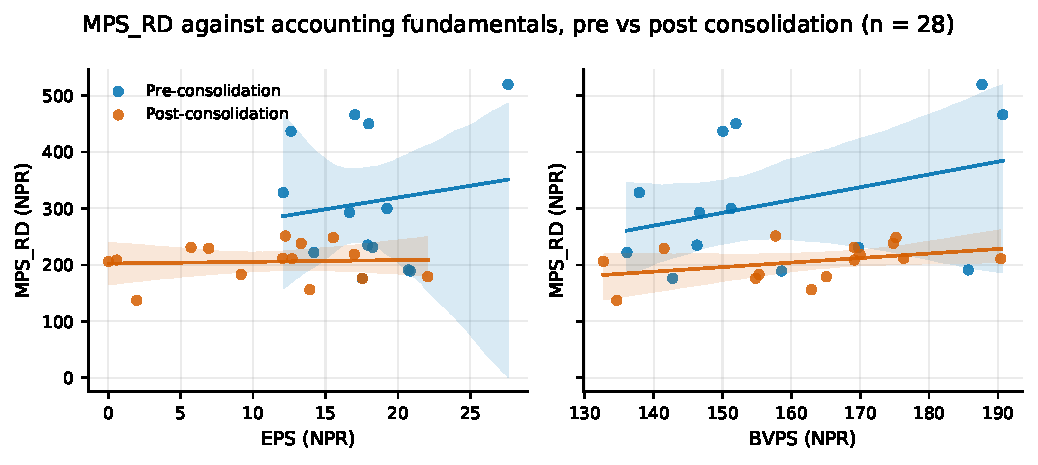
\includegraphics[width=0.92\textwidth]{figures/F3_value_relevance.pdf}
\caption{$\mathit{MPS}^{RD}$ against Fundamentals Pre vs.\ Post Consolidation}
\label{fig:value_relevance}
\vspace{2pt}
\begin{minipage}{\linewidth}
\footnotesize
\textit{Note.} Scatter panels and OLS regression lines of $\mathit{MPS}^{RD}$ against EPS (left) and BVPS (right), partitioned into pre-consolidation (FY 2076/77--2078/79, blue) and post-consolidation (FY 2079/80--2081/82, vermillion) sub-periods ($N = 28$) (Codebase Asset F3). Lines are descriptive bivariate OLS fits, not the two-way fixed-effects estimates in Table~\ref{tab:t4_model2}; the post-BVPS sign difference is the effect of absorbing year effects.
\end{minipage}
\end{figure}

\begin{figure}[!htbp]
\centering
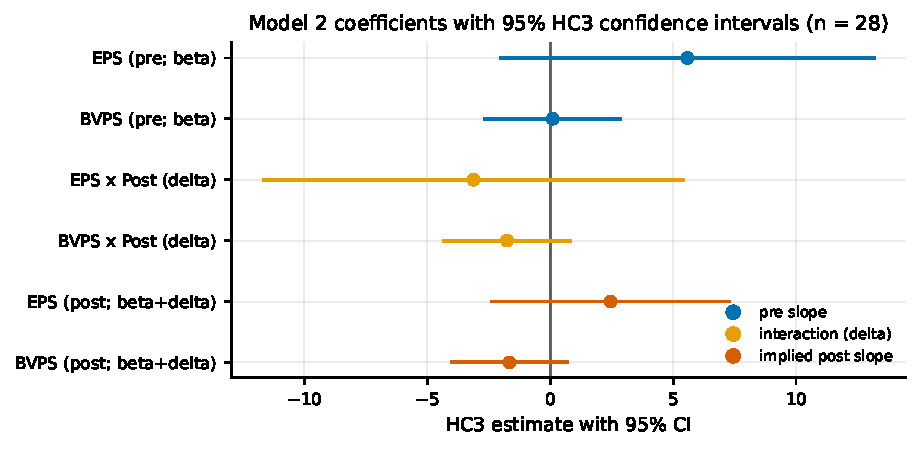
\includegraphics[width=0.88\textwidth]{figures/F4_coefficient_forest.pdf}
\caption{Model 2 Coefficients and 95\% HC3 Confidence Intervals}
\label{fig:coeff_forest}
\vspace{2pt}
\begin{minipage}{\linewidth}
\footnotesize
\textit{Note.} Coefficient forest plot displaying pre-consolidation slopes ($\beta_E, \beta_B$), interaction shifts ($\delta_E, \delta_B$), and implied post-consolidation linear combinations ($\beta_E+\delta_E, \beta_B+\delta_B$) from Model~2, estimated with MacKinnon-White HC3 robust 95\% confidence intervals on Student's $t(14)$ distribution ($N = 28, \text{residual df} = 14$) (Codebase Asset F4).
\end{minipage}
\end{figure}

\subsection{Hypothesis Testing}
Based on the econometric estimates obtained from Model~1 and Model~2, the four operational research hypotheses formulated in Chapter~I are formally evaluated at the designated two-tailed 5\% significance level ($\alpha = 0.05$).

To ensure rigorous transparency, Hypotheses $H_1$ and $H_2$ are evaluated under both Model~1 (overall six-year baseline slopes) and Model~2 (pre-consolidation regime slopes). In both specifications, the empirical decision is identical.

Table~\ref{tab:hypotheses} summarizes the formal hypothesis testing decisions.

\begin{table}[!htbp]
\centering
\small
\caption{Summary of Operational Hypothesis Testing Decisions}
\label{tab:hypotheses}
\begin{tabular}{>{\raggedright\arraybackslash}p{0.125\textwidth}>{\raggedright\arraybackslash}p{0.11\textwidth}>{\raggedright\arraybackslash}p{0.11\textwidth}cc>{\raggedright\arraybackslash}p{0.11\textwidth}>{\raggedright\arraybackslash}p{0.18\textwidth}}
\toprule
\textbf{Hypothesis} & \textbf{Model / Term} & \textbf{Null ($H_0$)} & \textbf{Estimate} & \textbf{$p$-value} & \textbf{Decision} & \textbf{Inference} \\
\midrule
$H_1$ (Model 1) & $\beta_E$ (Overall) & $\beta_E = 0$ & 2.095 & 0.616 & Fail to Reject & Positive slope; insignificant under $t(16)$. \\
\addlinespace
$H_1$ (Model 2) & $\beta_E$ (Pre Slope) & $\beta_E = 0$ & 5.577 & 0.140 & Fail to Reject & Substantial slope; insignificant at 5\% ($t(14)$). \\
\addlinespace
$H_2$ (Model 1) & $\beta_B$ (Overall) & $\beta_B = 0$ & 0.219 & 0.908 & Fail to Reject & Insignificant under $t(16)$. \\
\addlinespace
$H_2$ (Model 2) & $\beta_B$ (Pre Slope) & $\beta_B = 0$ & 0.100 & 0.940 & Fail to Reject & Indistinguishable from zero under $t(14)$. \\
\addlinespace
$H_3$ & $\delta_E$ (EPS Shift) & $\delta_E = 0$ & $-3.124$ & 0.448 & Fail to Reject & Downward shift; insignificant under $t(14)$. \\
\addlinespace
$H_4$ & $\delta_B$ (BVPS Shift) & $\delta_B = 0$ & $-1.758$ & 0.175 & Fail to Reject & Downward shift; insignificant under $t(14)$. \\
\addlinespace
Joint Test & Joint Wald & $\delta_E=\delta_B=0$ & $F=2.95$ & 0.085 & Fail to Reject & Marginal at 10\%; fails 5\% threshold. \\
\bottomrule
\end{tabular}

\vspace{4pt}
\begin{minipage}{\linewidth}
\footnotesize
\textit{Note.} All tests evaluated at $\alpha = 0.05$ (two-tailed $t$-tests for individual parameters; right-tail $F$-test for joint hypothesis). Estimates derived from Model~1 ($N = 28, \text{residual df} = 16$) and Model~2 ($N = 28, \text{residual df} = 14$) with two-way fixed effects and MacKinnon-White HC3 robust standard errors on Student's $t$ distribution.
\end{minipage}
\end{table}

Detailed evaluations of individual hypotheses:
\begin{enumerate}
    \item \textbf{Hypothesis 1 ($H_1$): Value Relevance of Earnings per Share:}
    \textit{Hypothesis Statement:} There is a statistically significant relationship between earnings per share and market share price ($H_0: \beta_E = 0$ vs.\ $H_1: \beta_E \ne 0$).
    In Model~1, the overall EPS slope is $\hat{\beta}_E = 2.095$ with an HC3 standard error of $4.096$ ($t = 0.51, p = 0.616$). In Model~2, the pre-consolidation EPS slope is estimated at $\hat{\beta}_E = 5.577$ with an HC3 standard error of $3.560$ ($t = 1.57, p = 0.140$). In both models, the point estimates are positive and economically meaningful, but because $p > 0.05$, the study fails to reject the null hypothesis of no statistical association at the 5\% significance level.
    \item \textbf{Hypothesis 2 ($H_2$): Value Relevance of Book Value per Share:}
    \textit{Hypothesis Statement:} There is a statistically significant relationship between book value per share and market share price ($H_0: \beta_B = 0$ vs.\ $H_1: \beta_B \ne 0$).
    In Model~1, the overall slope is $\hat{\beta}_B = 0.219$ ($t = 0.12, p = 0.908$). In Model~2, the pre-consolidation BVPS slope is $\hat{\beta}_B = 0.100$ with an HC3 standard error of $1.306$ ($t = 0.08, p = 0.940$). Because $p \gg 0.05$ across both specifications, the study fails to reject the null hypothesis. Prior to consolidation, book value per share provided negligible explanatory power for share prices beyond earnings and fixed effects.
    \item \textbf{Hypothesis 3 ($H_3$): Structural Shift in Earnings Value Relevance:}
    \textit{Hypothesis Statement:} The value relevance of earnings per share underwent a statistically significant shift following the 2023 consolidation wave ($H_0: \delta_E = 0$ vs.\ $H_1: \delta_E \ne 0$).
    The interaction coefficient is $\hat{\delta}_E = -3.124$ with an HC3 standard error of $4.003$ ($t = -0.78, p = 0.448$). Although the point estimate indicates a substantial downward shift in the valuation multiple, the individual coefficient is not statistically significant at conventional thresholds. The study fails to reject the null hypothesis of no structural shift in EPS value relevance when evaluated in isolation.
    \item \textbf{Hypothesis 4 ($H_4$): Structural Shift in Book Value Relevance:}
    \textit{Hypothesis Statement:} The value relevance of book value per share underwent a statistically significant shift following the 2023 consolidation wave ($H_0: \delta_B = 0$ vs.\ $H_1: \delta_B \ne 0$).
    The interaction coefficient is $\hat{\delta}_B = -1.758$ with an HC3 standard error of $1.231$ ($t = -1.43, p = 0.175$). Although the negative shift reduces the implied post-consolidation slope to $-1.658$, the interaction term does not achieve statistical significance at the 5\% level. The study fails to reject the null hypothesis of no structural shift in BVPS value relevance when evaluated in isolation.
    \item \textbf{Principal Joint Structural Test:}
    Evaluating the joint composite hypothesis $H_0: \delta_E = \delta_B = 0$ yields $F(2, 14) = 2.954$ ($p = 0.085$). While the study cannot reject the null hypothesis of parameter stability at the strict 5\% level, the marginal significance ($p < 0.10$) is consistent with non-trivial joint adjustments across accounting valuation multiples.
\end{enumerate}

\subsection{Robustness and Sensitivity Analyses (R1 through R8)}
To evaluate the stability of baseline estimates against alternative empirical assumptions, variable definitions, and sample compositions, an eight-specification suite comprising the two baseline models (R1--R2) and six robustness variants (R3--R8) was estimated. All specifications maintain two-way bank and fiscal-year fixed effects and MacKinnon-White HC3 robust inference on Student's $t$ residual degrees of freedom.

Table~\ref{tab:t5_robustness} summarizes the estimation results across the robustness suite, reporting point estimates, standard errors for both main slopes and interaction terms, and the joint Wald $F$-test.

\begin{table}[!htbp]
\centering
\small
\caption{Robustness and Sensitivity Analysis Across Econometric Specifications}
\label{tab:t5_robustness}
\setlength{\tabcolsep}{4pt}
\begin{tabular}{>{\raggedright\arraybackslash}p{0.19\textwidth}>{\raggedright\arraybackslash}p{0.13\textwidth}>{\raggedright\arraybackslash}p{0.12\textwidth}>{\raggedright\arraybackslash}p{0.14\textwidth}>{\raggedright\arraybackslash}p{0.12\textwidth}>{\raggedright\arraybackslash}p{0.12\textwidth}c}
\toprule
\textbf{Specification} & \textbf{Earnings (SE)} & \textbf{BVPS (SE)} & \textbf{$\delta_E$ (SE)} & \textbf{$\delta_B$ (SE)} & \textbf{Wald $F$ ($p$)} & \textbf{$n$} \\
\midrule
\textbf{R1:} Model 1 Baseline & 2.095 (4.096) & 0.219 (1.858) & --- & --- & --- & 28 \\
\addlinespace
\textbf{R2:} Model 2 Baseline & 5.577 (3.560) & 0.100 (1.306) & $-3.124$ (4.003) & $-1.758$ (1.231) & 2.95 (0.085) & 28 \\
\addlinespace
\textbf{R3:} ROA Replaces EPS & 83.760 (79.852) & 0.358 (1.381) & $-43.570$ (83.671) & $-1.901$ (1.290) & 2.46 (0.121) & 28 \\
\addlinespace
\textbf{R4:} Model 2 + DPS & 6.183 (4.508) & $-0.642$ (1.378) & $-4.072$ (5.151) & $-1.770$ (1.335) & 2.77 (0.100) & 28 \\
\addlinespace
\textbf{R5:} Excl.\ Transition & 5.993 (4.635) & $-0.201$ (1.849) & $-2.578$ (5.521) & $-1.880$ (1.419) & 2.41 (0.139) & 23 \\
\addlinespace
\textbf{R6:} Excl.\ Mismatch & 4.336 (3.724) & 0.802 (1.328) & $-2.436$ (4.755) & $-2.611$ (1.517) & \textbf{5.82 (0.021)\textsuperscript{*}} & 23 \\
\addlinespace
\textbf{R7:} Bonus-Adjusted & 5.775 (4.145) & 0.153 (1.632) & $-4.043$ (4.446) & $-1.533$ (1.595) & 2.37 (0.130) & 28 \\
\addlinespace
\textbf{R8:} Restated EPS & 5.256 (3.016) & 0.031 (1.300) & $-2.860$ (3.807) & $-1.812$ (1.223) & 2.92 (0.087) & 28 \\
\bottomrule
\end{tabular}

\vspace{4pt}
\begin{minipage}{\linewidth}
\footnotesize
\textit{Note.} \textsuperscript{*} Significant at $p < 0.05$. All models estimated by OLS with bank and fiscal-year fixed effects; MacKinnon-White HC3 robust standard errors reported in parentheses. The joint Wald $F$-statistic tests $H_0: \delta_E = \delta_B = 0$ under the MacKinnon-White HC3 covariance matrix. R3: ROA substitutes for EPS. R4: Cash DPS included (residual df = 13). R5: Transition year FY 2079/80 dropped ($N = 23, \text{residual df} = 10$). R6: FY 2078/79 entity-timing mismatch dropped ($N = 23, \text{residual df} = 10$). R7: BVPS adjusted for proposed bonus share capitalization ($\mathit{BVPS}_{\text{adj}} = \mathit{BVPS} / (1 + \text{bonus ratio})$, a pro-forma forward capitalization adjustment). R8: Restated basic EPS substituted for GBIME FY 2076/77 and NMB FY 2077/78 ($N = 28$). Residual degrees of freedom: R1 16; R2, R3, R7, R8 14; R4 13; R5, R6 10.
\end{minipage}
\end{table}

The sensitivity analysis yields critical econometric and substantive insights:
\begin{enumerate}
    \item \textbf{Operating Profitability Substitution (R3):} Substituting ROA (PAT divided by average total assets) for EPS yields an operating profitability slope of $83.760$ (HC3 SE = 79.852, $p = 0.312$) and an interaction shift of $\delta_{ROA} = -43.570$ (HC3 SE = 83.671, $p = 0.611$). The book value interaction remains negative ($\delta_B = -1.901, \text{SE} = 1.290, p = 0.163$), and the joint Wald test yields $F(2, 14) = 2.46$ ($p = 0.121$). This confirms that the observed valuation dynamics are not an artifact of per-share earnings scaling, but reflect fundamental operational repricing.
    \item \textbf{Dividend Incorporation (R4):} Augmenting Model~2 with declared cash dividends per share (DPS) produces an earnings slope of $\hat{\beta}_E = 6.183$ (SE = 4.508, $p = 0.193$) and a book value slope of $\hat{\beta}_B = -0.642$ (SE = 1.378, $p = 0.649$). The interaction shifts remain consistently negative ($\delta_E = -4.072, \text{SE} = 5.151, p = 0.443; \delta_B = -1.770, \text{SE} = 1.335, p = 0.208$), and the joint Wald $F$ is $2.77$ ($p = 0.100$). Because adding DPS consumes an additional parameter, residual degrees of freedom decrease from 14 to exactly 13 on $N = 28$.
    \item \textbf{Transition-Year Exclusion (R5):} Dropping the initial post-merger integration year (FY 2079/80, $N = 23, \text{residual df} = 10$) to eliminate one-off transition accounting friction preserves the structural pattern: $\hat{\beta}_E = 5.993$ (SE = 4.635, $p = 0.225$), $\hat{\delta}_E = -2.578$ (SE = 5.521, $p = 0.650$), $\hat{\delta}_B = -1.880$ (SE = 1.419, $p = 0.215$), with joint Wald $F(2, 10) = 2.41$ ($p = 0.139$). This pattern is consistent with the interpretation that the negative interaction shifts are not solely driven by temporary integration write-offs in the immediate post-merger fiscal year.
    \item \textbf{Entity-Timing Mismatch Exclusion (R6) --- Key Sensitivity Finding:} Specification R6 excludes FY 2078/79 ($N = 23, \text{residual df} = 10$). As established in Chapter~III, FY 2078/79 represents an entity-timing asymmetry: audited financial statements published at the end of Chaitra 2079 BS reflected standalone, pre-merger banking operations (ending mid-July 2022), whereas secondary market share prices observed on 13 April 2023 reflected the expanded, post-merger capitalized entities following early-2023 amalgamations.
    When this entity-mismatch fiscal year is excluded, the joint Wald test of regime shift becomes \textbf{statistically significant at the 5\% level}: \textbf{$F(2, 10) = 5.82, p = 0.021$}.
    In this FY 2078/79-excluded specification, the book value interaction shift is estimated at $\hat{\delta}_B = -2.611$ with an HC3 standard error of $1.517$ ($t = -1.72, p = 0.116$ on $t(10)$), while the earnings interaction is $\hat{\delta}_E = -2.436$ (HC3 SE = 4.755, $t = -0.51, p = 0.620$). While neither individual interaction term achieves significance at the 10\% level under the Student's $t(10)$ distribution, the joint test indicates that removing the entity-timing asymmetry yields a statistically significant joint structural difference across the pre- and post-consolidation calendar regimes.
    \item \textbf{Bonus Capitalization Adjustment (R7):} Adjusting book value for subsequent bonus share dilution ($\mathit{BVPS}_{\text{adj}} = \mathit{BVPS} / (1 + \text{bonus ratio})$) yields estimates virtually identical to baseline: $\hat{\beta}_E = 5.775$ (SE = 4.145, $p = 0.185$), $\hat{\delta}_E = -4.043$ (SE = 4.446, $p = 0.379$), $\hat{\delta}_B = -1.533$ (SE = 1.595, $p = 0.353$), with Wald $F(2, 14) = 2.37$ ($p = 0.130$).
    \item \textbf{Restated Earnings per Share (R8):} Substituting restated basic EPS (accounting for bonus issues in subsequent fiscal periods for GBIME FY 2076/77 and NMB FY 2077/78) leaves the baseline conclusions intact: $\hat{\beta}_E = 5.256$ (SE = 3.016, $p = 0.103$), $\hat{\delta}_E = -2.860$ (SE = 3.807, $p = 0.465$), $\hat{\delta}_B = -1.812$ (SE = 1.223, $p = 0.161$), with Wald $F(2, 14) = 2.92$ ($p = 0.087$).
\end{enumerate}

Figure~\ref{fig:robustness_forest} presents a coefficient forest plot summarizing parameter estimates and confidence intervals for the earnings channel across seven robustness specifications (R1, R2, and R4 through R8).

\begin{figure}[!htbp]
\centering
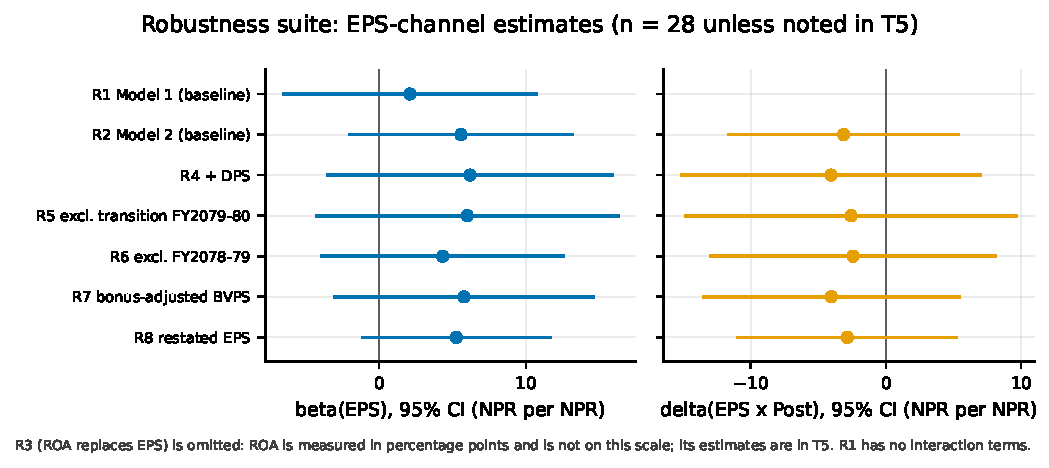
\includegraphics[width=0.92\textwidth]{figures/A2_robustness_forest.pdf}
\caption{Robustness Forest Plot Across Seven Specifications (R1, R2, R4--R8)}
\label{fig:robustness_forest}
\vspace{2pt}
\begin{minipage}{\linewidth}
\footnotesize
\textit{Note.} Forest plot of the EPS-channel estimates (earnings coefficient and EPS $\times$ Post interaction) with 95\% HC3 confidence intervals across seven specifications (R1, R2, R4--R8; R3 omitted because ROA is on a different scale; $N = 28$ or $N = 23$) (Codebase Asset A2).
\end{minipage}
\end{figure}

\subsection{Econometric Diagnostics and Specification Comparison}
To verify that the empirical findings are robust to potential violations of Gauss-Markov and asymptotic assumptions, a comprehensive battery of econometric diagnostics was performed.

Table~\ref{tab:t6_diagnostics} presents the diagnostic test statistics for the baseline model.

\begin{table}[!htbp]
\centering
\small
\caption{Econometric Diagnostics for Baseline Value-Relevance Model}
\label{tab:t6_diagnostics}
\begin{tabular}{>{\raggedright\arraybackslash}p{0.22\textwidth}cccc}
\toprule
\textbf{Diagnostic Dimension} & \textbf{Statistic} & \textbf{Value} & \textbf{$p$-value / Threshold} & \textbf{Assessment} \\
\midrule
VIF (EPS) & VIF & 1.16 & $< 10.0$ (Tolerance = 0.862) & Passed \\
\addlinespace
VIF (BVPS) & VIF & 1.16 & $< 10.0$ (Tolerance = 0.862) & Passed \\
\addlinespace
Breusch-Pagan Heteroskedasticity & LM & 14.37 & $p = 0.213$ ($\chi^2(11) = 19.68$) & Passed \\
\addlinespace
Cook's Distance (Influential) & Max $D_i$ & 0.552 & Cutoff: $4/N = 0.143$ & Addressed via HC3 \\
\bottomrule
\end{tabular}

\vspace{4pt}
\begin{minipage}{\linewidth}
\footnotesize
\textit{Note.} Diagnostics computed on Model~1 baseline ($N = 28$). Variance Inflation Factor (VIF) computed exclusively on substantive regressors (fixed effects dummies excluded). Breusch-Pagan Lagrange Multiplier test evaluates residual variance constancy across fitted values and regressors. Cook's distance evaluated using the correct parameter count ($K = 12$) against standard finite-sample threshold $4/N = 4/28 = 0.143$.
\end{minipage}
\end{table}

Key diagnostic findings:
\begin{enumerate}
    \item \textbf{Multicollinearity:} The variance inflation factors for EPS and BVPS are identical at $\text{VIF} = 1.16$ (tolerance = 0.862). Because these values fall well below the conventional conservative ceiling of $5.0$ (and standard threshold of $10.0$), multicollinearity between the substantive accounting fundamentals does not distort parameter estimation.
    \item \textbf{Heteroskedasticity:} The Breusch-Pagan test yields an LM statistic of $14.37$ ($p = 0.213$). Although the null hypothesis of constant error variance is not formally rejected at the 5\% level, all inferences throughout this dissertation are executed under MacKinnon-White HC3 standard errors, which provide asymptotic and finite-sample protection against arbitrary heteroskedasticity and high-leverage points.
    \item \textbf{Influential Observations:} Evaluating Cook's distance against the benchmark threshold $4/N = 4/28 = 0.143$ identifies five observations exceeding the cutoff, with a sample maximum Cook's $D$ of $0.552$ (HBL FY 2076/77). These high-leverage observations correspond to extreme price realizations during the 2021 NEPSE bull market. Deployment of HC3 standard errors explicitly addresses this leverage: the HC3 estimator divides squared residuals by $(1 - h_{ii})^2$, inflating high-leverage residuals to offset their artificially small OLS residuals. This yields conservative standard error estimates and protects inference against leverage distortion, without artificially trimming or modifying observed sample data.
\end{enumerate}

Figure~\ref{fig:diagnostics} presents the four-panel econometric diagnostic plot for Model~1 (Normal Q-Q, Residuals vs.\ Fitted, Scale-Location, and Cook's Distance).

\begin{figure}[!htbp]
\centering
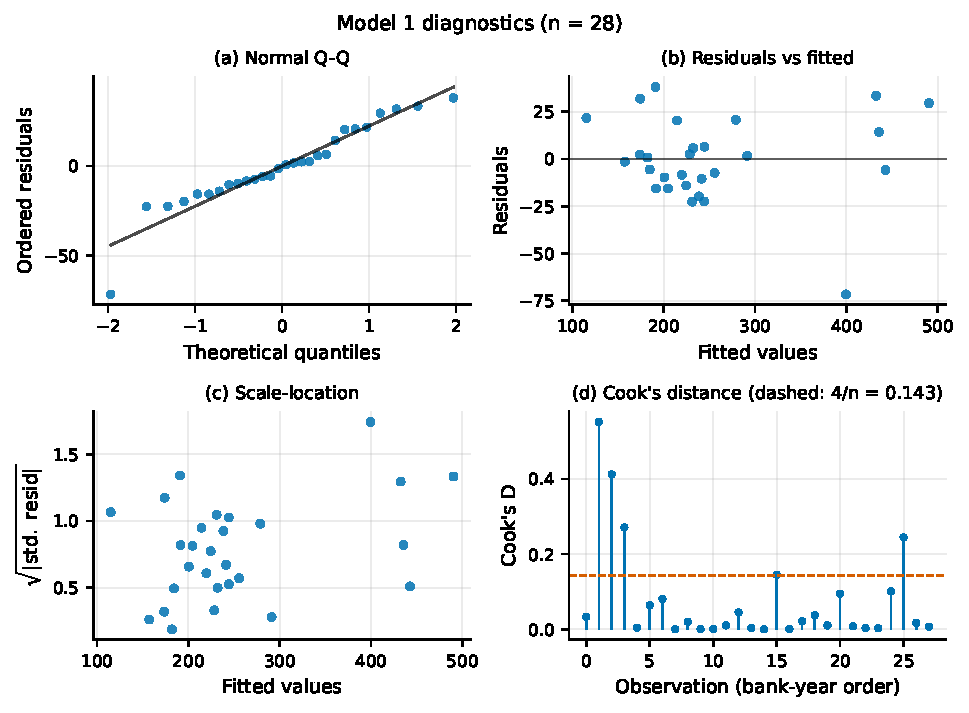
\includegraphics[width=0.92\textwidth]{figures/F5_diagnostics.pdf}
\caption{Econometric Residual Diagnostics for Baseline Model (Model 1)}
\label{fig:diagnostics}
\vspace{2pt}
\begin{minipage}{\linewidth}
\footnotesize
\textit{Note.} Four-panel diagnostic suite for Model~1: (top-left) Normal Q-Q plot assessing error normality; (top-right) Residuals vs.\ Fitted values assessing linearity; (bottom-left) Scale-Location plot ($\sqrt{|\text{standardized residuals}|}$ vs.\ fitted) assessing homoskedasticity; (bottom-right) Cook's distance across observations ($N = 28$) identifying leverage points against $4/N = 0.143$ (Codebase Asset F5).
\end{minipage}
\end{figure}

\subsubsection{Specification Comparison: Pooled OLS vs.\ Fixed Effects}
To demonstrate why two-way fixed effects estimation is the preferred econometric specification, Table~\ref{tab:spec_comp} compares parameter estimates across three nested specifications: Pooled OLS (no fixed effects), Bank Fixed Effects Only, and Two-Way Fixed Effects (Model~1).

\begin{table}[!htbp]
\centering
\small
\caption{Specification Comparison Across Econometric Model Structures}
\label{tab:spec_comp}
\setlength{\tabcolsep}{4pt}
\begin{tabular}{>{\raggedright\arraybackslash}p{0.18\textwidth}cccc>{\raggedright\arraybackslash}p{0.20\textwidth}}
\toprule
\textbf{Specification} & \textbf{$\beta_E$ (EPS Coef.)} & \textbf{$\beta_B$ (BVPS Coef.)} & \textbf{$R^2$} & \textbf{Resid.\ df} & \textbf{Assessment} \\
\midrule
Pooled OLS (No FE) & 4.882 (3.099) & 0.552 (1.259) & 0.136 & 25 & Conflates market cycles with relevance. \\
\addlinespace
Bank FE Only & 5.217 (5.360) & 1.432 (2.727) & 0.176 & 21 & Ignores macro-temporal price collapse. \\
\addlinespace
Two-Way FE (Model 1) & 2.095 (4.096) & 0.219 (1.858) & 0.948 & 16 & Rigorously absorbs bank and year shocks; preferred benchmark. \\
\bottomrule
\end{tabular}

\vspace{4pt}
\begin{minipage}{\linewidth}
\footnotesize
\textit{Note.} MacKinnon-White HC3 robust standard errors reported in parentheses. Dependent variable: $\mathit{MPS}^{RD}$. Analysis sample $N = 28$.
\end{minipage}
\end{table}

The comparison in Table~\ref{tab:spec_comp} reveals that Pooled OLS yields inflated point estimates ($\hat{\beta}_E = 4.882, \hat{\beta}_B = 0.552$) while explaining only 13.6\% of price variance ($R^2 = 0.136$). When fiscal-year dummies are added in the two-way fixed effects model, the explanatory power jumps to 94.8\% ($R^2 = 0.948$), while the estimated slopes attenuate to $\hat{\beta}_E = 2.095$ and $\hat{\beta}_B = 0.219$. This illustrates that in unadjusted pooled regressions, accounting fundamentals can easily absorb broader macroeconomic cycles, monetary policy shifts, and NEPSE-wide liquidity trends. However, it is noteworthy that even in the pooled specification, the EPS coefficient ($\hat{\beta}_E = 4.882, \text{SE} = 3.099, t = 1.58, p = 0.126$) is not statistically significant under HC3 robust inference.

\section{Discussion}

\subsection{Value Relevance of Accounting Fundamentals in the Pre-Consolidation Regime}
As reported in Table~\ref{tab:t4_model2}, in the pre-consolidation regime (FY 2076/77 through FY 2078/79), the estimated valuation multiple for earnings per share was $\hat{\beta}_E = 5.577$ ($p = 0.140$ on $t(14)$), whereas the multiple for book value per share was $\hat{\beta}_B = 0.100$ ($p = 0.940$ on $t(14)$).

Although these parameter estimates do not achieve conventional statistical significance at the 5\% level---a direct consequence of small-sample degrees of freedom ($N = 28$, residual $\text{df} = 14$) combined with conservative HC3 standard errors---their relative magnitudes provide valuable economic insights into the functioning of the Nepalese secondary banking market prior to the 2023 consolidation wave:
\begin{enumerate}
    \item \textbf{Dominance of Earnings over Book Value:} The substantial positive magnitude of $\hat{\beta}_E$ ($5.58$) relative to $\hat{\beta}_B$ ($0.10$) indicates that before the consolidation wave, equity investors on NEPSE prioritized current operational profitability and earnings generation over historical balance-sheet equity backing. In an equity market characterized by high retail participation and dividend anticipation, reported net profit per share served as the primary benchmark for valuing commercial banking equities. Investors viewed earnings as a direct indicator of immediate cash dividend paying capacity and bonus share distribution potential.
    \item \textbf{Economic Logic of Book Value Disregard:} The near-zero coefficient for book value per share ($\hat{\beta}_B = 0.100$) indicates that balance-sheet net worth exerted virtually no incremental pricing influence beyond earnings and fixed effects. Prior to 2023, Nepalese commercial banks operated in a regulatory regime where minimum paid-up capital had been escalated to NPR 8.0 billion pursuant to NRB's 2015 directive, but solvency and institutional viability were largely taken for granted by market participants. As long as banks maintained stable credit growth, low reported non-performing loan ratios, and predictable dividend streams, equity investors paid minimal attention to the underlying net asset backing, treating book value as an uninformative historical accounting construct.
\end{enumerate}

\subsection[Regime Shift: Earnings Deterioration and Book Value Multiples Post-Consolidation]{Regime Shift: Earnings Deterioration and Book Value Multiples Post-\\Consolidation}
As detailed in Table~\ref{tab:t4_model2}, following the consolidation wave of early 2023, the empirical estimates reveal a noticeable contraction in valuation multiples, with negative interaction coefficients ($\hat{\delta}_E = -3.124, p = 0.448; \hat{\delta}_B = -1.758, p = 0.175$) and attenuated implied post-consolidation slopes ($\hat{\beta}_E + \hat{\delta}_E = 2.453, p = 0.298; \hat{\beta}_B + \hat{\delta}_B = -1.658, p = 0.161$).

Because neither individual interaction term achieves statistical significance at conventional thresholds, and the joint Wald test in the baseline sample is marginally significant at 10\% ($p = 0.085$), these patterns are interpreted not as proven causal effects, but as suggestive structural tendencies consistent with several economic and institutional mechanisms operating in Nepal's post-merger banking environment:
\begin{enumerate}
    \item \textbf{Asset Quality Pressures and Loan Provisioning (Plausible Mechanism):} The horizontal amalgamations executed in 2023 required surviving commercial banks to assimilate legacy loan portfolios from acquired institutions. Contemporaneous industry reports and NRB supervisory data indicate that following consolidation, commercial banks experienced rising non-performing loans \citep{nrb2023list}, driven by broad macroeconomic deceleration, construction sector stress, and stricter loan-loss provisioning requirements. As credit-loss charges expanded, reported accounting earnings exhibited higher volatility and transitoriness. Equity investors may have recognized that reported net income was increasingly sensitive to provisioning assumptions, leading to a discount on earnings multiples. This mechanism is consistent with the observed drop in the earnings multiple, though direct asset quality variables are not estimated in the econometric model.
    \item \textbf{Capital Expansion and Share Supply:} Amalgamations significantly expanded the paid-up equity base of surviving banks through share swap agreements. The influx of newly created equity shares diluted per-share earnings (mean EPS contracted by 40.11\% post-consolidation, from NPR 17.90 to NPR 10.72) and expanded the secondary market float. Market participants may have factored this enlarged equity supply into their pricing models, anticipating slower growth in per-share metrics.
    \item \textbf{Dividend Cessation and Information Loss:} In the pre-consolidation period, regular cash dividends provided an observable benchmark for equity valuations (mean DPS = NPR 6.06). Following consolidation, regulatory capital conservation guidelines and heightened provisioning mandates coincided with widespread cash dividend suspensions (mean DPS fell to NPR 1.40, with 12 of 15 post-consolidation bank-years recording zero cash dividends). The withdrawal of regular dividend payments removed an observable cash flow signal, coinciding with the broader attenuation of earnings relevance.
    \item \textbf{Interpreting the Negative Book Value Point Estimate:} The negative implied slope for book value per share ($\hat{\beta}_B + \hat{\delta}_B = -1.658$, HC3 SE = 1.120, $t = -1.48, p = 0.161$) is statistically insignificant under the Student's $t(14)$ distribution. It cannot therefore be presented as an established empirical law. Econometrically, it reflects an exploratory point estimate indicating that post-consolidation book equity increases did not translate into proportional share price premiums. Conceptually, in a banking sector navigating complex post-merger integrations, expanded balance-sheet capital can reflect equity issued to absorb stressed assets or unamortized restructuring costs rather than unencumbered tangible net worth. Investors may have treated book equity expansion with caution, rather than as an unambiguous indicator of liquidation value.
\end{enumerate}

\subsection{Reconciling with Theoretical Frameworks}
The empirical findings can be evaluated against foundational theoretical models in accounting and financial economics:
\begin{enumerate}
    \item \textbf{Divergence and Resonance with \citet{kwon2020}:}
    Comparing our results with the post-merger valuation framework of \citet{kwon2020} reveals an important divergence alongside a shared insight:
    \begin{itemize}
        \item \textit{Where our results resonate:} In line with Kwon and Wang, our findings are consistent with the perspective that corporate amalgamations can introduce accounting noise and structural disruption that attenuate the valuation relevance of earnings. Following major mergers, financial statement comparability is disrupted, historical earnings predictability diminishes, and equity markets discount reported earnings multiples ($\hat{\delta}_E = -3.124$).
        \item \textit{Where our results diverge:} In Kwon and Wang's framework, when earnings become noisy following mergers, book value typically assumes an anchoring role, serving as a reliable proxy for net asset backing. In our Nepalese commercial banking sample, book value conspicuously did \textit{not} serve as an asset anchor; instead, its valuation multiple compressed from $\hat{\beta}_B = 0.100$ to an implied post-consolidation slope of $-1.658$. Unlike non-financial corporations, commercial banks cannot be readily evaluated on an orderly liquidation basis because they are subject to statutory resolution regimes and regulatory intervention.
    \end{itemize}
    \item \textbf{The \citet{ohlson1995} Residual Income Framework:}
    The Ohlson model specifies firm equity value as the sum of contemporaneous book value and capitalized expected future abnormal earnings:
    \begin{equation}
    P_t = B_t + \sum_{\tau=1}^{\infty} R^{-\tau} \mathbb{E}_t [\tilde{x}_{t+\tau}^a]
    \end{equation}
    Our baseline estimates in the pre-consolidation period display positive point estimates for both components ($\hat{\beta}_E = 5.58, \hat{\beta}_B = 0.10$). However, the post-consolidation regime exposes the limitations of linear valuation models during periods of banking restructuring. When clean-surplus accounting is complicated by merger reserve adjustments, swap accounting, and dividend halts \citep{collins1997}, linear pricing dynamics break down, producing wide confidence intervals and parameter attenuation.
    \item \textbf{Dividend Signaling Theory \citep{bhattacharya1979,john1985}:}
    Under dividend signaling theory, cash distributions provide a costly and credible signal verifying reported earnings quality. In the Nepalese banking sector, where retail equity investors face informational opacity regarding loan classifications, cash dividends historically functioned as an observable verification of accounting profits. When regulatory capital constraints forced banks to eliminate cash dividends post-consolidation, the absence of this verification signal coincided with the compression of the earnings valuation multiple.
    \item \textbf{Banking Opacity and Regulatory Forbearance \citep{morgan2002,flannery2004}:}
    Commercial banks are recognized in financial economics as opaque institutions due to the proprietary nature of loan assets and the discretion inherent in loan provisioning. In Nepal, regulatory forbearance provisions---allowing consolidated banks extended timelines to meet regulatory ratios---may have increased informational opacity. When market participants cannot independently verify loan portfolio quality, they discount reported accounting metrics, widening standard errors and attenuating valuation slopes.
\end{enumerate}

\subsection{Comparative Context with Nepalese and International Empirical Studies}
Evaluating the empirical findings of this dissertation against prior literature reveals important methodological and empirical distinctions:
\begin{enumerate}
    \item \textbf{Methodological Differences with Prior Nepalese Studies:}
    Prior empirical literature on Nepalese commercial banks has predominantly reported large, statistically significant positive coefficients for accounting fundamentals \citep{bhattarai2014,bhandari2026,joshi2023}. In contrast, our two-way fixed effects baseline yields statistically insignificant slopes ($\hat{\beta}_E = 2.10, p = 0.616; \hat{\beta}_B = 0.22, p = 0.908$). This divergence reflects four critical methodological factors:
    \begin{itemize}
        \item \textit{Exclusion of Circular Price-to-Earnings Multiples:} Several prior Nepalese studies included the Price-to-Earnings (P/E) ratio as an explanatory regressor predicting share price \citep{bhattarai2014,chhetri2023,giri2024,joshi2023,pant2024}. As demonstrated mathematically in Chapter~II, because $\text{P/E} = \mathit{MPS} / \mathit{EPS}$, regressing $\mathit{MPS}$ on P/E introduces the dependent variable into the regressor, generating mechanical circularity and inflated statistical significance. This dissertation strictly excludes P/E.
        \item \textit{Omission of Macro-Year Fixed Effects in Pooled Models:} Prior studies frequently relied on pooled OLS or one-way random effects, omitting fiscal-year dummies. As our specification comparison in Table~\ref{tab:spec_comp} illustrates, pooled OLS yields an inflated point estimate ($\hat{\beta}_E = 4.882$) compared to two-way fixed effects ($\hat{\beta}_E = 2.095$). In unadjusted pooled regressions, accounting fundamentals can inadvertently absorb broad macroeconomic cycles and the severe post-2021 NEPSE market correction. When year fixed effects absorb market-wide price levels, slope coefficients reflect strictly within-year cross-sectional variation. Notably, even in our pooled specification, HC3 robust inference yields an insignificant slope ($t = 1.58, p = 0.126$), confirming that the lack of significance is not an artifact of fixed effects alone, but reflects genuine estimation uncertainty.
        \item \textit{Standardized Reporting-Deadline Measurement:} Prior studies commonly measured share prices at fiscal year-end (Ashadh-end / mid-July), long before audited reports were published. By measuring share prices strictly at the post-reporting-deadline statutory window under Section 59(2) of BAFIA, operationalized at the end of Chaitra (mid-April) \citep{bafia2017}, this study eliminates look-ahead bias and ensures that audited accounting numbers were legally public.
        \item \textit{Sample Harmonization:} In reconciling prior samples, \citet{bhattarai2014} analyzed nine commercial banks over 2006--2014, while \citet{joshi2023} analyzed seven commercial banks over 2012/13--2021/22. Both examined pre-consolidation periods under pooled structures, explaining their higher reported significance.
    \end{itemize}
    \item \textbf{Alignment with Recent Methodological Studies:}
    Our findings closely parallel more recent Nepalese studies that document valuation instability:
    \begin{itemize}
        \item \citet{chaudhari2025} examined ten commercial banks over 2014/15--2023/24 without P/E circularity and documented unstable valuation relationships, finding that traditional financial ratios lost predictive power during recent macroeconomic stress.
        \item \citet{pant2024} investigated seven commercial banks through FY 2023/24 and documented a negative, statistically insignificant BVPS coefficient, consistent with our post-consolidation findings.
        \item \citet{timalsina2026} observed that bank share prices decoupled from historical accounting metrics following the post-2023 liquidity contraction.
    \end{itemize}
    \item \textbf{Emerging Market Literature Context:}
    In broader emerging and frontier markets, studies such as \citet{almumani2014} in Jordan and \citet{malhotra2013} in India demonstrate that during periods of regulatory disruption and financial sector reform, accounting value relevance tends to decline. Frontier equity markets appear highly sensitive to structural transitions, with accounting numbers losing pricing power during periods of institutional restructuring.
\end{enumerate}

\subsection{Methodological Context: Transition Dynamics and Structural Discontinuities}
The sensitivity analyses conducted in Section~4.2.6 provide important methodological insights for evaluating corporate restructuring in frontier capital markets:
\begin{enumerate}
    \item \textbf{Entity-Boundary Timing and Sensitivity Check R6:}
    The most salient sensitivity finding arises from specification R6, which excludes FY 2078/79 ($N = 23, \text{residual df} = 10$). In that specification, the joint Wald test of regime shift achieves statistical significance at the 5\% level:
    \begin{equation}
    F(2, 10) = 5.82, \quad p = 0.021
    \end{equation}
    This result highlights an institutional timing feature of corporate combinations. In FY 2078/79, audited financial statements reflected the pre-merger standalone operations of the legacy banks (for the fiscal year ending mid-July 2022), whereas secondary market share prices observed on 13 April 2023 reflected the enlarged, merged entities following amalgamations in January--February 2023. When this entity-mismatch year is included, the baseline joint test does not reject structural stability at the 5\% level ($p = 0.085$). After excluding this mismatch year, the joint test rejects parameter stability at the 5\% level ($p = 0.021$). The evidence for a regime shift is therefore suggestive in the baseline and statistically significant in the sensitivity check; it is reported as an empirical association across calendar regimes, rather than as a causal merger effect.
    \item \textbf{The 5-Day Freshness Rule and Trading Suspensions:}
    The exclusion of HBL and NIMB for FY 2077/78 highlights an institutional friction in Nepalese capital markets. Secondary market trading remained suspended across extended merger processes, suspending price discovery for weeks or months. Dropping observations that exceeded the 5-day freshness window rather than imputing stale pre-suspension prices was essential to maintaining empirical integrity.
    \item \textbf{BAFIA Section 59(2) Reporting Deadlines as an Empirical Anchor:}
    Anchoring share price observations to the nine-month statutory reporting deadline under Section 59(2) of BAFIA, operationalized at the end of Chaitra (mid-April), provided an objective, reproducible observation window grounded in Nepalese banking law, eliminating the measurement ambiguity of unverified announcement dates while avoiding look-ahead bias.
\end{enumerate}

In summary, the empirical results indicate that commercial bank valuations in Nepal exhibited noticeable shifts across the 2023 consolidation wave. Valuation multiples on earnings compressed and book value multiples turned negative, reflecting an environment characterized by increased earnings transitoriness, dividend reductions, and asset quality challenges. While baseline models show suggestive joint shifts, statistical significance emerges once entity-boundary timing mismatches are resolved, highlighting the critical importance of temporal alignment in empirical valuation research.

